% CPSC 438 Final Project Paper
% Christopher Chute, David Brandfonbrener, Leo Shimonaka, Matthew Vasseur

% Author and Title Information
\newcommand*{\thetitle}{Scalability Limits of HDFS}
\newcommand*{\theauthor}{Christopher Chute, David Brandfonbrener, Leo Shimonaka, Matthew Vasseur}
\newcommand*{\duedate}{May 3, 2016}

% Document Settings
\documentclass[11pt, a4paper]{article}
\author{\theauthor}
\title{\thetitle}
\date{\duedate}
\usepackage[top=.75in, left=0.5in, right=0.5in, bottom=1.5in]{geometry}
\usepackage{amsmath, amsthm, amssymb}
\newtheorem{lem}{Lemma}
\usepackage{graphicx}
\usepackage{setspace}
\usepackage{enumitem}
\usepackage{booktabs}
\usepackage[T1]{fontenc}
\usepackage{titling}

% Multicolumn Formatting
\usepackage{multicol}
\setlength\columnsep{18pt}    % spacing between columns

\setlength{\droptitle}{-9em}
\posttitle{\par\end{center}\vspace{-.35em}}

% Header Formatting
\usepackage{fancyhdr}
\setlength{\headheight}{48pt}
\pagestyle{fancyplain}
%\lhead{\thetitle}
%\rhead{\theauthor\\\duedate}
%\rfoot{}
\cfoot{\thepage}

% ************************* End of Preamble ***********************
\begin{document}
\maketitle
\thispagestyle{empty}

\begin{abstract}
    This paper explores the scalability limits of the Hadoop Distributed File System (HDFS). The single-machine, in-memory metadata store of HDFS is a known bottleneck for applications requiring storage of many small files. This architecture presents other theoretical bottlenecks, including CPU load on the NameNode from storing many small files. For example, both high-frequency requests and heartbeats with small files require higher NameNode CPU usage. In this paper we model and provide experimental evidence for the NameNode memory bottleneck. We compare this to proposed CPU bottlenecks, and we find that the memory bottleneck is the dominant issue. We provide suggestions for future work on HDFS scalability limits.
\end{abstract}
\begin{multicols*}{2}


\section{Introduction}

Distributed filesystems (DFS), also known as network filesystems, store remote files in a format accessible with the same semantics as a local filesystem. A DFS offers a transparent interface for handling files and directories, access control, recovery and concurrency. Additionally, a DFS offers a scalable mechanism for creating logical filesystems shared by many clients.

The DFS architecture has many advantages: it offers a unified hierarchical namespace for shared files and folders, location transparency in physical data placement, load balancing across nodes, storage scalability via expanding clusters, increased availability through distributed data, and fault tolerance by replication across racks.

Many DFS implementations exist today. Each system differs in their performance, data mutability, management of concurrent writes, failure handling, and storage policies. These include POSIX-compliant systems like Lustre, search-engine enhanced Google File System (GFS), and non-proprietary open-source DFSs like Hadoop Distributed File System.

This paper examines Hadoop Distributed File System (HDFS), a module of the Apache Hadoop ecosystem. HDFS is a distributed filesystem focused on scalability and portability. HDFS is not fully POSIX-compliant, specifically designed for handling large files terabytes in size. It trades the POSIX functionality like mutable files for increasing data throughput and supporting operations like Append.

The architecture of HDFS is designed with the following goals in mind \cite{HdfsGuide}:
\begin{enumerate}[noitemsep, label=\arabic*.]
	\item\textit{Support regular hardware failures.} Data is replicated across multiple DataNodes for fault tolerance.
	\item\textit{Allow streaming data access.} Partitioning is transparent so that files appear to be stored sequentially. Reads are distributed so that streaming access does not block other transactions.
	\item\textit{Support very large data sets.} To provide scalability, more DataNodes can be added to support large data sets. This assumes that the NameNode memory limit will not become a bottleneck before the disk space of the DataNodes.
	\item\textit{Provide simple concurrency control.} In HDFS's write-once, read-many model, only one appender/creator per file is allowed at a given time. Written data is immutable. This allows HDFS to provide highly available and concurrent reads.
	\item\textit{Run everywhere (portability).} HDFS runs on top of the Java Virtual Machine, which provides nearly universal portability.
\end{enumerate}

HDFS's key characteristic is how it decouples metadata from file data. Although its centralized namespace storage offers several advantages for linear performance scaling, it also introduces hard bounds for growth. This paper explores how these limitations occur, analyzes its objective effects on performance, and discusses potential approaches to overcoming this limit.

The rest of this paper is organized as follows. In section 2, we outline the architecture of a HDFS cluster. Section 3 provides a high-level overview of how this architecture interferes with the system's performance. Section 4 discusses the design and analysis of various experiments conducted on an HDFS cluster, followed by proposals on ways to improve performance in Section 5. Section 6 concludes.
% -------------------------------------------------

\end{multicols*}

\begin{center}
	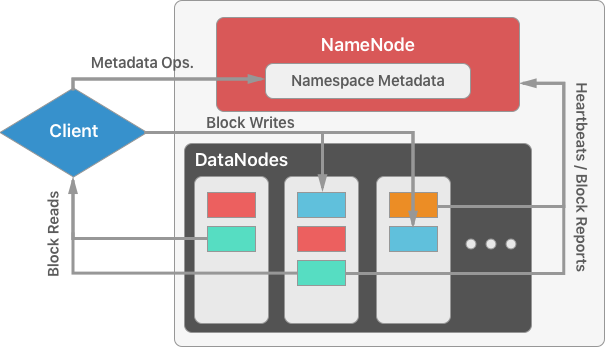
\includegraphics[keepaspectratio=true, width=0.75\textwidth]{Architecture}\\
	\textit{Fig. 1: Architecture of HDFS}
\end{center}

\begin{multicols*}{2}
\section{HDFS Architecture}
With these principles in mind, the HDFS architecture is designed as follows. Much of the information in this section is adapted from \cite{HdfsArch}. A HDFS cluster consists of a single NameNode and many DataNodes. Briefly, the NameNode holds the metadata for each file in the file system. Metadata for a directory consists of an inode, and metadata for a file consists of an (inode, mapping) pair. The inode is a UNIX-style inode and thus contains properties such as permissions and ownership. Moreover, an HDFS inode stores HDFS-specific attributes such as quotas and replication factors.

Each file is partitioned into one or more blocks, and each block is replicated across multiple DataNodes. The mapping for a file maps each block of the file to a list of DataNodes where the block is replicated. As presented in Section \ref{MetadataSize}, the metadata associated with each file scales linearly with the number of blocks in each file. That is, there is a fixed size mapping for each block in the file. The NameNode holds all of this metadata in memory to facilitate fast metadata operations.

A single NameNode is used primarily to simplify the architecture and metadata management of HDFS. For instance, having a single NameNode makes it simpler to maintain consistency in the file system. A single NameNode architecture also allows for simple, centrally organized replication of each block across many DataNodes. If the metadata was not centralized, this replication operation and updating all data mappings would become complicated, and potentially overuse the network connecting the nodes.

All metadata is kept in memory on the NameNode. Given a file of size $F$ and a block size $B$, the file will be partitioned into $n = \lceil F/B\rceil$ blocks. Upon creation of the file, the NameNode replicates each of the $n$ blocks across $R$ DataNodes, where $R$ is the \textit{replication factor} of the cluster. Once the file is created, the NameNode is responsible for pointing read or append requests to the appropriate blocks on the DataNodes. The NameNode keeps the block mappings up-to-date by communicating with the DataNodes via \textit{block reports} carried in periodic heartbeats from each DataNode. A heartbeat also indicates that a DataNode is functioning correctly and has a working network connection. The NameNode uses this information to ensure each block is replicated over $R$ DataNodes, issuing replication commands if needed.

Durability of the NameNode is critical to the availability of HDFS. There are various schemes to ensure a durable NameNode. A write-ahead log is maintained on stable storage and this can be used to build a BackupNode or CheckpointNode that essentially maintains a copy of the NameNode. By default, the NameNode is a single point of failure for an HDFS cluster, and reconstructing the NameNode after failure involves sending 

Files in HDFS are append-only and can only be written to by a single writer at a time. That is, once data is written it cannot be overwritten. This simplifies concurrency control and allows the system to guarantee that writes can be read as soon as a file is closed. On a write, a client must first query the NameNode to find which DataNodes and blocks to write. Then, the client will ensure a replicated write by sending packets of data through a pipeline of TCP connections. This pipeline includes all DataNodes over which the file will be replicated, which guarantees that the writes will be consistent across multiple DataNodes. On a read, a client must first query the NameNode to find which DataNodes contain replicas of the desired file and which blocks hold the file. Then, the client reads from the closest available DataNodes directly.

\section{Scalability Limits}\label{ScalabilityLimits}
Despite the benefits of having only a single NameNode, this architectural decision limits the scalability of HDFS. These problems are especially pronounced when HDFS is used to store many small files as opposed to few large files. In particular, a single file must be partitioned into at least one block, even if its entire contents are less than the block size. Thus even small files produce a block mapping of metadata. As a result, small files produce more metadata relative to their content size. This exhausts the available memory of the NameNode even for moderately sized data sets when they consist of many small files. This memory bottleneck has been discussed in the literature, notably in \cite{HdfsScale}. For this same reason, small files result in larger block reports as each DataNode can hold a larger number of (virtual) blocks. Finally, the high-frequency access pattern associated with small files causes increased interaction with the NameNode, which creates another potential bottleneck.

\subsection{Physical Memory Size}
% Re-iterate in-memory metadata namespace
% Total File Capacity of Cluster is Limited by Name Node's RAM due to requirement that all metadata objects (file inodes and block) in memory at all times
% SHVACHKO PAPER EXAMPLE: Assuming on average, a file consists of \lambda = 1.5 blocks, then each file uses 1 file and ~2 data block objects, hence uses ~600 bytes. Thus to keep 100 million files, name-node must have at least 60GM of RAM

In this section we present an analysis of the memory bottleneck described above.

\subsubsection{Theoretical Model}

Let $ M $ be the size of memory on the NameNode in bytes, $ \lambda $ be the number of blocks allocated to each file, and $ F $ be the number of files on the system. Also, let $ c $ be the number of bytes to represent a single block mapping to all replicas of a block, and $i$ the number of bytes to represent and inode. If we want to fit all metadata into memory, it is clear that we must have:
\begin{align*}
	M > \lambda c F + i F
\end{align*}
This limit is much easier to reach with small files since each file is allocated its own virtual block, no matter how small the file is, \textit{i.e.,} we have that $ \lambda \geq 1$. This means that creating many small files should take up $ c + i$ bytes for each additional file, while growing a file by a similar amount will use at most $ c $ bytes. Thus, the memory limit is much more of a problem for many small files. 
	
\subsubsection{Simulation}

Using this model, we can perform simulations of how much data can be stored in an HDFS cluster if each file is of a given size. The motivation for this is that with larger files, each file will use more blocks, and thus create more metadata. However, the cost of storing the inode relative to the amount of data in the file will decrease with larger files. It is interesting to see how both file size and block size affect the total amount of data that an HDFS cluster can store before the memory bottleneck is reached.
	
Below, we have graphs that represent the outcomes of these simulations. We assume that the NameNode has 2GB of RAM, and we perform the simulation for various block sizes (the size of each block that a file is divided into). We use the metadata sizes of $c = i = 150$, approximating our experimental findings below. First, we ran the simulation with a block size of 128 MB. We have one plot of file sizes from 1 byte to 100 GB and another showing only file sizes larger than the block size of 128 MB, since this part is nonlinear and more interesting. 
\begin{center}
	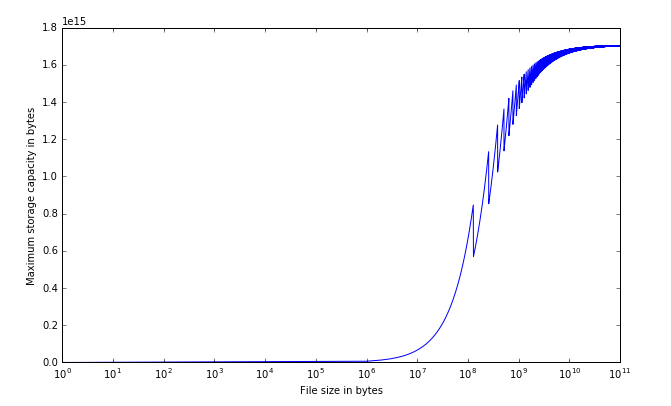
\includegraphics[keepaspectratio=true, width=0.45\textwidth]{logScale}
	\textit{Fig. 2: Cluster Capacity vs. File Size}
\end{center}

\begin{center}
	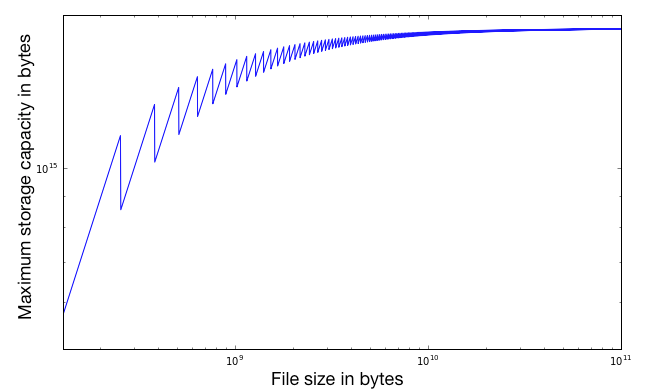
\includegraphics[keepaspectratio=true, width=0.45\textwidth]{logLogScale}
	\textit{Fig. 3: Capacity vs. File Size (Zoomed Window)}	
\end{center}

While each file is smaller than one block, a file is always allocated its own block in the system and thus has a constant metadata size. Then, since the files are linearly increasing in the amount of data they hold, but metadata remains constant, the capacity of the system (as limited by the RAM on the NameNode) grows linearly until files are larger than blocks. 

Once a file is larger than a block, the behavior becomes more interesting. At the threshold where the file size increases from $n$ blocks to $n+1$ blocks, the cost of the extra metadata to record this block outweighs the increase in file size so that the overall capacity of the system decreases. This causes the zig-zag nature of the above graph. At the same time, the system also begins to reach the limit of the number of metadata mappings that can be stored in 2 GB, explaining why the graph flattens out with very large files. 

Lastly, we ran the same simulation with many different block sizes.  Since the block size determines the number of blocks per file, and thus the amount of metadata per file, a larger block size should create less metadata per file. This resulted in the following plot:
\begin{center}
	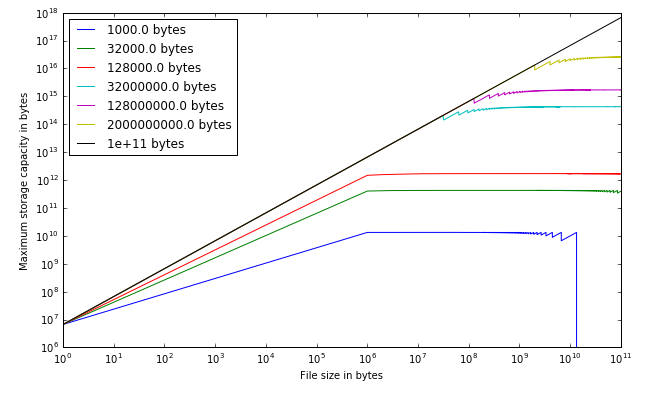
\includegraphics[keepaspectratio=true, width=0.45\textwidth]{variableBlockSize}	
	\textit{Fig. 4: Capacity vs. File Size (Varying Block Size)}
\end{center}

This graph shows how larger block size does indeed lead to larger system capacity. In fact the system has the highest capacity if each block is as large as memory of the NameNode, but such large blocks are impractical, as explained below. Another interesting point is that for the smallest block size, we see that at a certain point a single file that creates too many blocks will not fit in the system. Thus, the system has capacity 0. This happens since the metadata to hold all of the blocks for a single file of that size would not fit in memory on the NameNode. 

Thus, we expect this memory limit to be affected in the following main ways. (1) Larger files will give the system a larger overall capacity. (2) Larger blocks will give the system larger overall capacity, assuming the limiting factor is memory on the NameNode and not disk on the DataNodes (since we can always add more DataNode machines).

Although large blocks produce the smallest amount of metadata, increasing the block size poses a tradeoff. There are two primary concerns with a very large block size. First, a larger block size causes data to be less equally distributed throughout the cluster. This potentially reduces the efficiency of streaming reads, as file operations are less distributed across the DataNodes. Second, during a MapReduce job, each map task is run on a single block (the FileSplit factor is set to the size of a block) \cite{HdfsDefaults}. As a result, larger blocks make MapReduce less distributed and hence less efficient. In practice HDFS has a large default block size of 128 MB \cite{HdfsDefaults}.

\subsection{NameNode CPU Bottleneck}
The less obvious scalability problem with the HDFS architecture is the potential for a CPU bottleneck at the NameNode. The system is built on the assumption that metadata operations are inexpensive relative to network communication and file I/O. The HDFS architecture also assumes that there will be few enough large files that the number of such metadata operations (including requests for block locations) will be insignificant. However, with many small files, these assumptions are violated and the NameNode CPU could become a bottleneck.

% Describe the INTERNAL-LOAD communicating with DataNodes
% # of Heartbeats that NameNode receives is directly proportional to # of DataNodes in cluster
% # of Block reports is also directly proportional to size of data blocks (i.e. ratio of blocks mapped per file) and also # of replicated copies per block
% Physical data storage and data I/O performance increase proportionally to # of DataNodes in cluster and size of data blocks, but the overall performance of HDFS is also affected negatively by increased internal load.
% The more time spend on internal load, less time spend on processing external client's requests

The first potential source of CPU bottleneck is the internal-load of communication with the DataNodes. This internal-load can be created in two ways. First, internal-load can be created when the system holds a large amount of small files. The size of the block report sent by each DataNode is directly proportional to the number of blocks that the DataNode holds. Since each file is given its own virtual block even if the entire file is much smaller than a block, small files allow each DataNode to hold a larger number of blocks. That is, small files increase the block density. As a result, each DataNode must send a larger block report to the NameNode with each heartbeat. The processing of these block reports could potentially overload the NameNode CPU and increase the latency of requests to the NameNode.

% Describe the external load from clients
% All metadata operations run on Namenode - they cannot be processed anywhere else.
% On every file read, there is a get_block_location per block per file
% On every file write, there is a create_block per block per file
% Namenode can become a bottleneck with operations that involve many metadata operations, e.g. batch-write operations will include many create_block requests
% -------------------------------------------------
Another potential source of CPU bottleneck is external load from clients querying the NameNode. As explained above, for each read or write of a block, a client must query the NameNode to obtain the list of DataNodes where the block is replicated. The NameNode must then perform a metadata operation to determine what to return to the client. Therefore, the NameNode can become a bottleneck if there are many clients trying to perform operations concurrently since they all must access the metadata via the singular NameNode. This should be an especially prevalent problem when there are many small files because it would be likely that the use pattern of a system with many small files would be for there to be many clients each trying to access their files concurrently. Moreover, DataNode operations should return relatively quickly since each file operation is on a small amount of data. This I/O speedup may be mitigated by more disk seeks, due to the fact that I/O with small files is less sequential.

With these potential CPU bottlenecks in mind, we pose the question of whether it is reasonable to generate an appropriate load so as to reach these CPU bottlenecks before the NameNode runs out of memory. In our experiments we determine whether the CPU bottleneck is ever the dominant scalability limit for HDFS. We restrict our experiments to valid requests and simulate a plausible usage pattern for small files (\textit{e.g.,} each file requested must exist and there are no ``hot'' files).

\section{Performance Evaluation}
% Goals of the experiments
In this section we present our experimental results on the memory bottleneck and the CPU bottlenecks of HDFS. We evaluate HDFS 2.7.1 on a cluster consisting of four identical Amazon EC2 instances. Each instance has 8 GB of disk space, 2 GB of RAM, and a 3.3 GHz Intel Xeon processor. Three of these instances are dedicated as DataNodes, and one instance is the NameNode. Although this is a small amount of memory for a typical HDFS NameNode, the goals of our experiments are to analyze the performance of HDFS around the limits of memory. Thus we are concerned with the amount of metadata \textit{relative} to the capacity of the NameNode's memory, rather than the absolute amount of metadata. Our experimental results can be normalized to account for the memory capacity of the NameNode and the disk capacity of the DataNodes.

% Mention experimental setup (EC2, Java Test Skeleton, # nodes, etc)
We query HDFS using the Hadoop Java API. On top of the FileSystem class provided by the API, we implemented a class called HDFSClient. Each HDFSClient object is runnable, and represents a single client making file access or modification requests to the file system. On each machine querying the NameNode, we spin up a pool of threads, each of which wraps an HDFSClient and reads from a global thread-safe \textit{request queue}. The master thread (different in each experiment) generates requests and places them on the request queue for processing by the HDFSClient worker threads. Each client repeatedly removes a request from the queue, issues that request to the NameNode and waits for the subsequent response. Examples of requests include writing a file from the local file system to HDFS, reading a file from HDFS, and deleting a file from HDFS.

% FOR EACH EXPERIMENT:
% Discuss designs of individual experiments and their results
% What were the experiments testing?
% What were the different parameters of the experiments?
% Possibilities of error?
\subsection{Memory Bottleneck Experiments}
In this section we explore the memory bottleneck of HDFS. First we provide empirical results on the metadata size, and then we precisely determine when the NameNode will run out of memory.
\subsubsection{Experiment 1: Metadata Size}\label{MetadataSize}
The first goal of our experiments is to determine precisely how much memory is occupied on the NameNode for each file added to the system. Analysis of the source code for HDFS and theoretical results in the literature suggest that each file should yield roughly 150 bytes of inode plus 150 bytes for each block to account for the mapping \cite{HdfsArch, HdfsScale}. However, the peculiarities of the NameNode storage for recovery suggest that these numbers are not precisely correct. The NameNode stores the FSImage, a snapshot of the filesystem, as well as an Edits log that indicates the updates since the last snapshot. Backups of each file are also maintained. Hence it is possible that as more files are added to the system, each additional file will result in more occupied memory on the NameNode. Moreover we seek to verify that the mapping for each block is fixed-size, whether or not the entire block is occupied by file contents.

To test the size of metadata, we create a pool of HDFSClient threads and add large batches of files to HDFS (cf. MetadataSizeTest.java). We measure the resulting increase in occupied memory on the NameNode. We find that 
% TODO: Insert the metadata size results with graphs.

\subsubsection{Experiment 2: Memory Bottleneck}\label{MemoryBottleneck}
% TODO: Check the reported memory bottleneck results.
Next we pushed our HDFS cluster to the memory bottleneck. This was achieved by continually adding small files (10 B each) to the HDFS cluster until the write requests were refused. We found that our 2 GB NameNode could support roughly 234,000 10-byte files, accounting for approximately 112 MB of metadata. This discrepancy between 2 GB and 112 MB exists because the HDFS NameNode must run the Java Virtual Machine as well as a version of Linux. Thus the metadata storage was restricted to 112 MB of heap memory. This limit can be changed in the HDFS configuration and was set to its maximum value in our experiments given the size of our NameNode memory.

We note that once the memory bottleneck is reached, HDFS does not refuse more files but rather the JVM fails on basic operations. For example, a query of the root directory (\texttt{hdfs dfs -ls /}) fails due to shortage of memory. So the file system is rendered unreadable unless files are removed.

\subsection{CPU Bottleneck Experiments}\label{CPUBottleneck}
In this section we test the throughput of file operations as more files are added to HDFS. We analyze different request patterns to determine the performance bottleneck. We note that the small size of our cluster makes our results on throughput less convincing. That is, because there are only three DataNodes for the NameNode to monitor, there is relatively little block report processing on the NameNode CPU. Nonetheless, we can still add a large number of blocks and analyze throughput of HDFS near the memory limit.
\subsubsection{Experiment 3: Read Throughput}\label{ReadThroughput}
We next tested the throughput of HDFS reads as more small files were added to the system. One might expect throughput to decrease as more files are added due to the increasing complexity of block mappings, as well as a wider range of disk seeks on the DataNode. In this experiment (found in ThroughputTest.java), there is a pool of 64 HDFSClient workers on three different machines. The workers go through two stages: First we create a pool of worker threads and measure throughput while reading roughly 1000 random files from HDFS to the local file system. In the second stage, new workers add 25,000 files to the system. The worker threads are killed and the throughput is again measured with 25,000 additional files on the system. This was repeated at increments of 25,000 files until the memory bottleneck was reached at roughly 234,000 files.

We found that there was no decrease in throughput as more files were added. As shown in Figure 5, the read throughput hovered around 100 files per second. This supports the HDFS design assumption that metadata operations are inexpensive relative to other file system and network operations of HDFS. Moreover, it does not support the hypothesis that disk seeks on random file access are more expensive when more files were added.

\begin{center}
	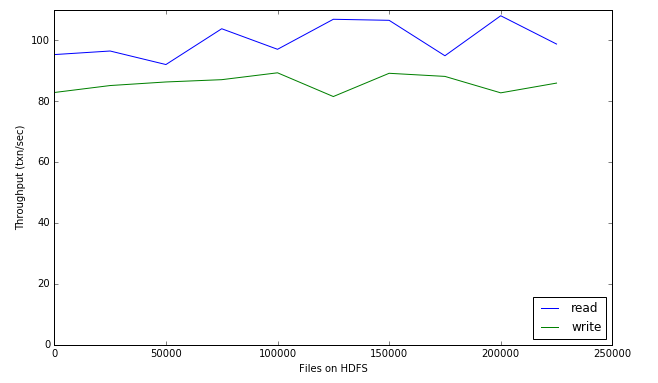
\includegraphics[keepaspectratio=true, width=0.45\textwidth]{ThroughputResults}
	\textit{Fig. 5: Isolated Read/Isolated Write Throughput}
\end{center}
\subsubsection{Experiment 4: Write Throughput}\label{WriteThroughput}
Although read throughput was not affected by the number of files stored on the cluster, we posited that write throughput may still be affected. While reads need only query a single DataNode, writes must be replicated down a pipeline of $R$ DataNodes, where $R$ is the replication factor (here $R = 3$). Hence write operations involve  all DataNodes in our cluster. Each DataNode must perform a disk seek to a free location in physical memory, and HDFS cannot select the least busy DataNode to service a request.

The design of the write throughput experiments mirrored the design of the read throughput test. As seen in Figure 5 above, our experiments showed no decrease in write throughput as more files are added to HDFS. The write throughput hovered around 80 files per second over the entire range of 0 to 225,000 files on the cluster.
% TODO: Insert graphs for write throughput.

\subsubsection{Experiment 5: Mixed Reads and Writes}\label{ReadWriteThroughput}
A more typical usage pattern for HDFS would involve interleaved reads and writes. Therefore we ran experiments measuring throughput of HDFS mixed reads and writes as more files are added to the system. We note that it is possible that batch writes allow each DataNode in the pipeline to avoid disk seeks between writes. That is, assuming there is a large contiguous segment of free disk space available, the DataNode can write each new file sequentially without disk seeks. Thus Experiment 4 above would not show any decrease in throughput due to disk seeks. However, mixed (random) reads and writes would force each DataNode to seek on disk, so one might still expect to see performance degenerate as more small files are added.

The results of our experiments showed that...
% TODO: Read/write experimental results.

\subsubsection{Experiment 6: High-Frequency Requests}\label{HighFrequencyRequests}
% Discuss raw results independently for each experiment:
% Are these results what was expected (and why)?
% If there was some error, discuss what may have caused it
% Graphs
% Evaluate experimental results holistically to pinpoint the problem with HDFS's Single Namenode architecture (I.e. weigh CPU and Memory problems against each other)
% -------------------------------------------------
A dataset consisting of a large number of small files would likely receive a higher frequency of queries than another dataset. A typical client will read a file, process that file's data, then request the next file. Small files will be processed at the client more quickly than large files, therefore one would expect the client to have a higher frequency of requests. Since each request must first query the NameNode for a block mapping, this will put a large strain on the NameNode. In this section we explore the possibility that this usage pattern associated with small files results in a bottleneck.

Our experimental setup was as follows. Again we used HDFSClient threads querying from multiple machines. We uploaded a large set of roughly 25,000 10-byte files to HDFS. The HDFSClients then randomly read these files to their local file system. We measured the throughput of these requests as the number of clients varied from a single connection thread and moving up to 64 HDFSClients. Each client made requests as quickly as possible, and we looked for a decrease in throughput as the NameNode received more concurrent read and write queries. This produced the following graph.
\begin{center}
	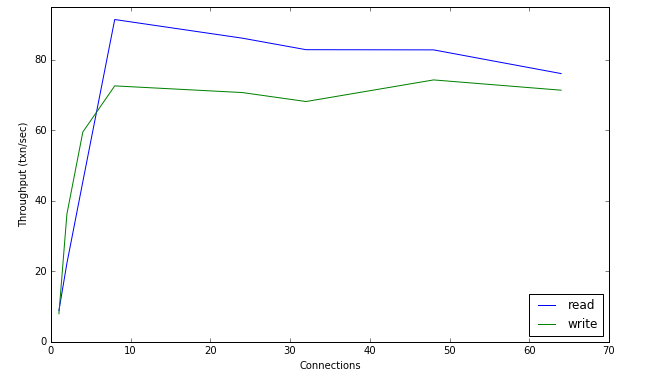
\includegraphics[keepaspectratio=true, width=0.45\textwidth]{ConcurrencyResults}	
	\textit{Fig. 6: Read Throughput vs. Request Frequency}
\end{center}
We see that there is an initial spike in throughput as the utilization of the DataNodes increases to full capacity. In the case of reads, there is a slight decrease in the number of connections beyond 8. Importantly we do not observe a sharp decline in throughput. For writes, we see no decline whatsoever.

These results show only that the scalability of reads and writes is not linear. That is, there is some bottleneck achieved around 8 connections. However, we expected that this bottleneck is not due to NameNode processing but rather in disk I/O and network communication between the DataNodes. To test this hypothesis, we ran the same test but only requested the block \textit{locations}. Thus the read and write requests never reached the DataNodes. This produced the following graph.
% TODO: Experiment where we only request the block locations.

\section{Improvements to Single NameNode Architecture}\label{Improvements}
% Use experimental data to determine what is actually detrimental to performance of HDFS, and suggest a way to improve it
% -------------------------------------------------
% Would it be helpful to remove the assumption that each file is assigned to its own block? Could be done with intermediate layer that puts small files into larger file, prevents edits

Some improvements have been suggested to solve the scalability problems with HDFS. One attempt to address the memory bottleneck is Apache's HDFS Federation. This system modifies HDFS by creating multiple NameNodes each of which has its own separate namespace \cite{Federation}. This is not a fundamental solution to the architectural problem, but rather merely adds more hardware to increase the memory bottleneck. Thus HDFS Federation is still a potentially inefficient use of memory on the NameNodes given a dataset of many small files. Additionally, with multiple independent namespaces the system cannot perform operations across the namespaces. Thus, the complexity of cross-partition transactions must be handled by the client application. The client can use symbolic links and client-side mount tables to make the multiple namespaces transparent to the user, so long as the client can tolerate higher request latency.

Some other distributed file systems like CalvinFS have been designed to more fundamentally address the memory bottleneck of the singular NameNode \cite{CalvinFS}. 

One potential new solution would be to add an intermediate layer if you knew that you had many small files that would only be written once and never appended. 
EXPLAIN THIS.

\section{Conclusion}

\bibliographystyle{plain}
\bibliography{citations.bib}
\end{multicols*}
\end{document}


























 ``